%
%   Chapter Related Works
%
%   Qing-Cheng Li (r01922024 at csie dot ntu dot edu dot tw)
%   R.O.C.103.07
%
\chapter{相關研究與文獻}
\label{c:related}

本章將分別介紹知識庫相關的資源與研究,
涵蓋了結構化知識庫(Structural Knowledge Base)、
知識庫加速(Knowledge Base Accerleration)與知識庫的應用(Application of Knowledge Base),
以及樣式與實體間關係的相關研究。

\section{知識庫}
\subsection{結構化知識庫}
相對於Wikipedia以文章來儲存知識,\cite{dbpedia} 的DBpedia、
\cite{yago} 的YAGO以及\cite{freebase} 的Freebase等都以結構化的方式儲存知識。
DBpedia、YAGO與Freebase都提供以TTL(Terse RDF\footnote{Resource Description Framework} Triple Language)格式儲存的資料,
以供處理與利用。

DBpedia是一個大型、多語言的知識庫,自Wikipedia擷取知識。
透過Wikipedia條目內的資訊框(Inforbox),擷取實體的特性,並連結實體。
並進一步整理了資訊框內的特性,以人工將語意相同的實體特性合併。

YAGO除了自Wikipedia擷取資訊外,還搭配了WordNet\footnote{http://wordnet.princeton.edu/},
建立一個輕量、高品質與覆蓋度的實體與關係資料庫。
其以<實體,關係,實體>的形式儲存事實(Facts),即實體與實體間的關係,
並定義關係的領域(Domain)與範圍(Range)、
階層式架構的實體類型(Types)與其他資源如DBpedia、WordNet間的連結。

Freebase是一個用以結構化人類知識的社群協作的可擴展元組(Scalable tuple)資料庫。
與Wikipedia一樣,是由志願者創建與維護其中的資料,並與其它知識庫亦互有連結。

\subsection{知識庫加速}

\cite{kba2012,kba2013}縱覽了2012、2013年的TREC知識庫加速競賽,
連續兩年都有的CCR(Cumulative Citation Recommendation)任務是過濾內容串流,
推薦對更新目標實體有幫助的文章,以縮短知識產生與知識庫更新之間的時間差。
圖\ref{i:kba-corps}是這兩年CCR任務中內容串流的資料量與目標實體的數量,
內容串流中每小時約有100,000份文件。
CCR任務主要專注在尋找文章中是否有出現目標實體(Mentions/Zero Mentions),
再進一步依照有幫助的程度分成四個等級(Garbage/Neutral/Useful/Vital)。

\begin{figure}
    \centering
    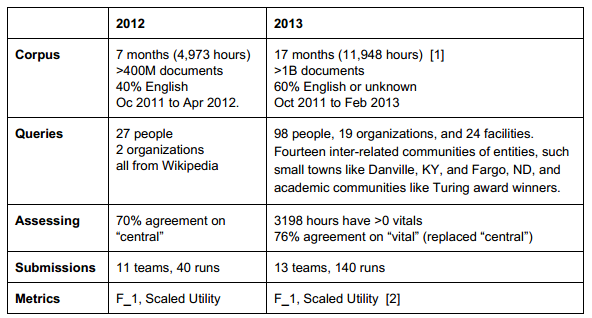
\includegraphics[width=0.65\textwidth]{images/02-kba-corpus}
    \caption{TREC知識庫加速競賽資料量}
    \label{i:kba-corps}
\end{figure}

\cite{kba-hltoce}是2012年效能最好的團隊,
以具名實體、單字詞(Unigram)作為特徵訓練SVM分類器,
對每個目標實體訓練一個二元分類器。
把尋找實體的問題作為主題分類(Topic Classification)問題來處理。

\cite{kba-msra}則是2013年效能最好的團隊。
以查詢擴展(Query Expansion)、分類與學習式排序法(Learning to rank)。
其中分類是使用以文件特徵、實體特徵、文件與實體特徵、
時間特徵與引用特徵訓練隨機森林(Random Forest)分類器。

此外,\cite{kba-entity-detection}也專注於尋找串流中的實體,
提出了當出現新的實體時不需要新的訓練資料集的方法。
使用了文件中心特徵、實體資料特徵與時間特徵訓練隨機森林分類器,
以尋找串流中與實體高度相關的文件。
並且以TREC KBA 2012的資料做測試,
效能比\cite{kba-hltoce}還要好。

\subsection{知識庫的應用}

知識庫的應用常見於問答系統或實體消歧義上。

在問答系統的應用上,知識庫提供了一個知識的集合,也就是答案的來源,
\cite{yago-qa}將問句轉換為查詢語言,對YAGO進行查詢並回答問題。
\cite{freebase-qa-extract}利用Freebase的資料,以邏輯形式(Latent Logical Forms)對映問題與答案。
\cite{freebase-qa-parse}將知識庫視為一個實體為點,關聯為邊的圖,
假設答案只會存在於周遭的節點上,成為一個主題圖(Topic Graph),
將問句剖析後在圖上走訪尋找答案。

而在具名實體消歧義(Named Entity Disambiguation)上的應用,
\cite{dbpedia-spotlight} 提供了一個系統將文本內的實體連結至DBpedia。
他們將DBpedia的實體建立向量空間模型(Vector Space Model),
但與傳統VSM不同的是,IDF(Inverse Document Frequency)反應一個字在整個資料集內的重要程度,
卻沒辦法反應一個字在歧義候選選項內的重要程度。
為了要能夠找出一個字對消歧義的能力,
他們提出ICF(Inverse Candidate Frequency)來取代IDF計算字在向量空間中的權重,
定義$ICF(word) = log \frac{|R|}{n(word)}$,其中$|R|$是候選實體的數量,
$n(word)$是字在候選實體中出現的次數。
將DBpedia的實體以向量空間模型建模,以$TF*ICF$計算字的權重,
將文句與候選的實體向量空間模型計算相似度,取最相似的作為真正的結果。

% 這個有點複雜呀Orz...
% \cite{freebase-google} 則是Google則利用Freebase對實體消歧義。

%
%   Pattern and Relation
%
\section{樣式與實體間關係}

實體間的關係是可能隨著時間而產生變化的,
知道哪些關係會變化對於協助知識庫的更新是有幫助的,可以更注意那些會變動的關係。
\cite{relationsByTime} 提到有些實體間的關係是相對恆常的,
例如《1Q84》的作者是村上春樹是不會改變的事實;
而有些關係則是隨著時間而變動的,例如美國的總統是布希,只有在某一段時間內是正確關係。
此研究將實體間的關係分為是否為恆常(Constant)或是否唯一(Unique)。
恆常是指是否這組關係不會隨著時間改變,唯一是指抽換實體後關係是否仍然正確。
此研究人工挑選1,000組關係並利用時間、實體出現在特定時段內的頻率、文法等特徵對關係進行分類。

在擷取關係的部分,
\cite{reverb} 建立了一套開放資訊擷取系統(Open Information Extraction System),
可以擷取開方式的關係<$arg_1$, $relation$, $arg_2$>,
而不限於人工標定的關係。
過去的開放式資訊擷取系統會有非相干擷取(Incoherent Extraction)或無資訊擷取(Uninformative Extraction)的問題,
透過句法限制(Syntactic Constraint),
制定由詞性標記所組成的正則表示式,例如圖\ref{i:reverb-pos},
定義關係可以出現的形式,避免非相干擷取的問題。
詞彙限制(Lexical Constraint)認為一個合法的關係應該在大型的語料庫之中會有許多不重複的參數(Argument)。
由大型語料庫中擷取出的關係中,不重複參數配對的數量超過一個定值才會被認為是合法的關係,
以解決無資訊擷取的問題。

\begin{figure}
    \centering
    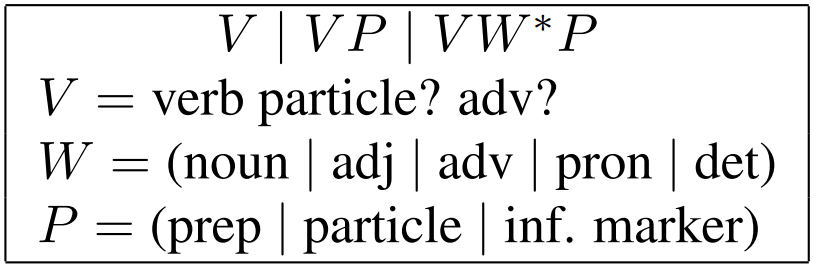
\includegraphics[width=0.45\textwidth]{images/02-reverb-pos}
    \caption{詞性標記組成的正則表示式}
    \label{i:reverb-pos}
\end{figure}

而Wikipedia中,每一篇文章,或稱條目,是描寫一個特定的實體,
\cite{wisenet} 自Wikipedia文章中提及其他實體的句子擷取關係,
由於同一種關係可能由不同的字樣來表達,為了建立同義字樣集,
定義了連結實體間關係的字樣間的相似度是字樣連結的實體重複的比例,
比例越高越相似,相似的字樣就可以聚集成同義字樣集,
並且應用Wikipedia的分類與上下文給予同義字樣集語意上的分類。

\cite{patty,patty2012}建立了一個名為PATTY的分類集(Taxonomy),
自Wikipedia、New York Times中擷取出樣式,建立同義樣式集(Pattern Synset),
並將同義樣式集合併,連結知識庫定義的實體關係。

PATTY的關係是以「<Domain> Pattern <Range>」表示,
Domain與Range是實體的類型(Types),來自知識庫YAGO、DBpedia。
而PATTY的樣式是以單字(Words)、詞性標記(Part-Of-Speech Tags)、萬用字元(Wildcards)所組成,
例如「<$person$>'s [adj] voice * <$song$>」中,
Domain是$person$,即第一個實體的類型是$person$;
Range是$song$,即第二個實體的類型是$song$ 。
「[adj]」是詞性標記,代表這裡可以填入任意形容詞,「voice」是單字,必須完全匹配,
「*」是萬用字元,可以填入任何字。
例如「Amy Winehouse's soft voice in `Rehab'」這個句子就符合這個樣式。

PATTY擷取樣式的方式是自Wikipedia、New York Times抽取句子,
以史丹佛剖析器(Stanford Parser\footnote{http://nlp.stanford.edu/software/lex-parser.shtml})對句子建立相依性剖析樹,
以YAGO、Freebase作為實體的字典,判斷若句子中有兩個實體,
則把兩實體間在樹上的最短路徑上的字句擷取出來作為樣式,
並進一步合併樣式為同義樣式集。
比起\cite{reverb},PATTY可以抽取任意的關係,不被詞彙或句法所限制。

抽取出樣式後,為了評估一個樣式的品質,PATTY定義了一個信心值(Confidence)。
對每一個樣式,都存在一組支持集(Support Set),
由符合樣式的實體對(Pairs of entites)所組成。
透過支持集的大小,對每個樣式計算信心值,
將樣式中的實體類別改為類別繼承架構中的更廣義的父節點類別,
以可以填入的實體對數作為分母,支持集作為分子,
得到的分數就是心信值,代表一個樣式的品質。

除了同義樣式集之外,PATTY還做了關係釋義(Relation Paraphrasing):
給定一個來自知識庫的關係,判斷一個樣式是否可以描述此一關係。
PATTY內有127,811個樣式可以描述225種DBpedia關係,43,124個樣式可以描述25種YAGO關係。
其透過隨機選取1,000組釋義來評估,平均的精確度(Precision)是0.76$\pm$0.03。

本研究欲使用樣式來尋找關係、實體特性,
PATTY正好提供了所需要的樣式,以及樣式可以描述哪些關係等資料。

